\documentclass[11pt, a4paper]{scrartcl}
\usepackage[
	typ=ab,
	fach=Informatik,
]{schule}

\usepackage{subfig}
\usepackage{inconsolata}

\title{Objekte am Raspberry Pi}

% % ================================
%        Pakete
% ================================

\usepackage[dvips, bottom=2.5cm, top=2.5cm, right=2.5cm, left=3cm]{geometry}
\usepackage[utf8]{inputenc}
\usepackage[ngerman]{babel}
\usepackage[babel,german=quotes]{csquotes}
\usepackage[T1]{fontenc}
\usepackage{enumerate}
\usepackage{setspace}
\usepackage{mdframed}
\setstretch{1.3} 
\setlength\parindent{0pt}
\usepackage{textcomp}
\usepackage{enumerate}
\usepackage{color}
\usepackage{graphicx}
\usepackage{colortbl}
\usepackage{hhline}
\usepackage{tabularx}
\usepackage{booktabs}
\usepackage[font={footnotesize}, labelfont=bf]{caption}
\usepackage[dvipsnames]{xcolor}
\usepackage{float}
\usepackage{subfig}
%\usepackage{hhline}
\usepackage{listings}

\renewcommand{\lstlistingname}{Quelltext} 

\definecolor{deepblue}{rgb}{0,0,0.5}
\definecolor{deepred}{rgb}{0.6,0,0}
\definecolor{deepgreen}{rgb}{0,0.5,0}



% ================================
%        Quelltexte JAVA
% ================================

% Java style for highlighting
\newcommand\javastyle{\lstset{
language=Java,
basicstyle=\ttfamily\scriptsize\mdseries,
otherkeywords={self},          
keywordstyle=\ttfamily\scriptsize\mdseries\color{deepblue},
emph={MyClass,__init__},          
emphstyle=\ttfamily\scriptsize\mdseries\color{deepred},   
stringstyle=\ttfamily\scriptsize\mdseries\color{deepgreen},
commentstyle=\ttfamily\scriptsize\mdseries\color{orange},
frame=,                         
showstringspaces=false,
showtabs=true, 
tabsize=3, 
tab=,
showstringspaces=false,
numbers=left,
extendedchars=true,
breaklines=true,
numberstyle=\tiny,
numbersep=9pt,
stepnumber=1,
captionpos=b,
backgroundcolor=\color[gray]{0.95},
}}

\newcommand\javastyleoneline{\lstset{
language=Java,
basicstyle=\ttfamily\scriptsize\mdseries,
otherkeywords={self},          
keywordstyle=\ttfamily\scriptsize\mdseries\color{deepblue},
emph={MyClass,__init__},          
emphstyle=\ttfamily\scriptsize\mdseries\color{deepred},   
stringstyle=\ttfamily\scriptsize\mdseries\color{deepgreen},
commentstyle=\ttfamily\scriptsize\mdseries\color{orange},
frame=,                         
showstringspaces=false,
showtabs=true, 
tabsize=3, 
tab=,
showstringspaces=false,
numbers=left,
extendedchars=true,
breaklines=true,
numberstyle=\tiny,
numbersep=9pt,
stepnumber=1,
captionpos=b,
backgroundcolor=\color[gray]{0.95},
belowcaptionskip=0em,
belowskip=0em,
}}

% Java for external files
\newcommand\javaexternal[2][]{{
\javastyle
\lstinputlisting[#1]{#2}}}

% Java for inline
\newcommand\javainline[1]{{\javastyle\lstinline!#1!}}



% ================================
%        Quelltexte Bash
% ================================

% Bash style for highlighting (ken Abstand unter der eingefügten Bash-Zeile)
\newcommand\bashstyleoneline{\lstset{
language=BASH,
basicstyle=\ttfamily\scriptsize\mdseries,
otherkeywords={self,bash,git},          
keywordstyle=\ttfamily\scriptsize\mdseries\color{deepblue},
emph={MyClass,__init__},          
emphstyle=\ttfamily\scriptsize\mdseries\color{deepred},   
stringstyle=\ttfamily\scriptsize\mdseries\color{deepgreen},
commentstyle=\ttfamily\scriptsize\mdseries\color{orange},
frame=,                         
showstringspaces=false,
showtabs=true, 
tabsize=3, 
tab=,
showstringspaces=false,
numbers=left,
extendedchars=true,
breaklines=true,
numberstyle=\tiny,
numbersep=9pt,
stepnumber=1,
captionpos=b,
backgroundcolor=\color[gray]{0.95},
belowcaptionskip=0em,
belowskip=0em,
}}

% normaler Bash Style
\newcommand\bashstyle{\lstset{
language=BASH,
basicstyle=\ttfamily\scriptsize\mdseries,
otherkeywords={self,bash,git},          
keywordstyle=\ttfamily\scriptsize\mdseries\color{deepblue},
emph={MyClass,__init__},          
emphstyle=\ttfamily\scriptsize\mdseries\color{deepred},   
stringstyle=\ttfamily\scriptsize\mdseries\color{deepgreen},
commentstyle=\ttfamily\scriptsize\mdseries\color{orange},
frame=,                         
showstringspaces=false,
showtabs=true, 
tabsize=3, 
tab=,
showstringspaces=false,
numbers=left,
extendedchars=true,
breaklines=true,
numberstyle=\tiny,
numbersep=9pt,
stepnumber=1,
captionpos=b,
backgroundcolor=\color[gray]{0.95},
}}

% Bash Style in schwarz
\newcommand\bashstyleblack{\lstset{
language=BASH,
basicstyle=\ttfamily\scriptsize\mdseries,
otherkeywords={self,bash,git},          
keywordstyle=\ttfamily\scriptsize\mdseries\color{black},
emph={MyClass,__init__},          
emphstyle=\ttfamily\scriptsize\mdseries\color{black},   
stringstyle=\ttfamily\scriptsize\mdseries\color{black},
commentstyle=\ttfamily\scriptsize\mdseries\color{black},
frame=,                         
showstringspaces=false,
showtabs=true, 
tabsize=3, 
tab=,
showstringspaces=false,
numbers=left,
extendedchars=true,
breaklines=true,
numberstyle=\tiny,
numbersep=9pt,
stepnumber=1,
captionpos=b,
backgroundcolor=\color[gray]{0.95}
}}

% BASH for external files
\newcommand\bashexternal[2][]{{
\bashstyle
\lstinputlisting[#1]{#2}}}

% BASH for inline
\newcommand\bashinline[1]{{\bashstyle\lstinline!#1!}}



\lstset{% 
	breaklines=true, % Zeilenumbrüche
	language=Java, % Sprache
	basicstyle=\ttfamily\small,
	commentstyle=\ttfamily\small\color{black!50},
	breakatwhitespace=false,
	tabsize=2,
	numbers=left, numberstyle=\footnotesize,  numbersep=5pt,
}

\begin{document}
%\pagestyle{empty}

\section*{Anschluss von Objekten an den Raspberry Pi}

Am Raspberry Pi können verschiedene Objekte angeschlossen werden. Dazu verfügt jedes Objekt über Anschlüsse, die auf dem Steckbrett mit dem GPIO des Raspberry Pi verbunden werden müssen. Dabei ist es wichtig, die Kabel so zu stecken, wie es die Anschlüsse auf dem Objekt vorschreiben.

Bei Anschlüssen mit der Aufschrift \enquote{3,3V} oder \enquote{GND} kann ein entsprechender ausgewählt werden. Dabei können an diese beiden Pinne auch mehrere Objekte angeschlossen werden.

Bei den anderen Aufdrucken, in den meisten Fällen \enquote{PIN}, kann am GPIO ein beliebiger \enquote{IO}-Pin ausgewählt werden. Bei diesem darf aber jeweils nur ein Objekt angeschlossen werden. Dieser Pin muss dann später im Programm angegeben werden, um z.\,B. das Objekt zu steuern oder den Zustand auszulesen.

In Abbildung \ref{fig:objekte_steckbrett} werden zwei Beispiele gegeben, wie die Objekte anzuschließen sind.

\begin{figure*}[htb]
     \subfloat[Anschluss des RGB-Scheinwerfers (Anschluss an ">IO02"<, ">IO03"<, ">IO04"< und ">GND"<).]{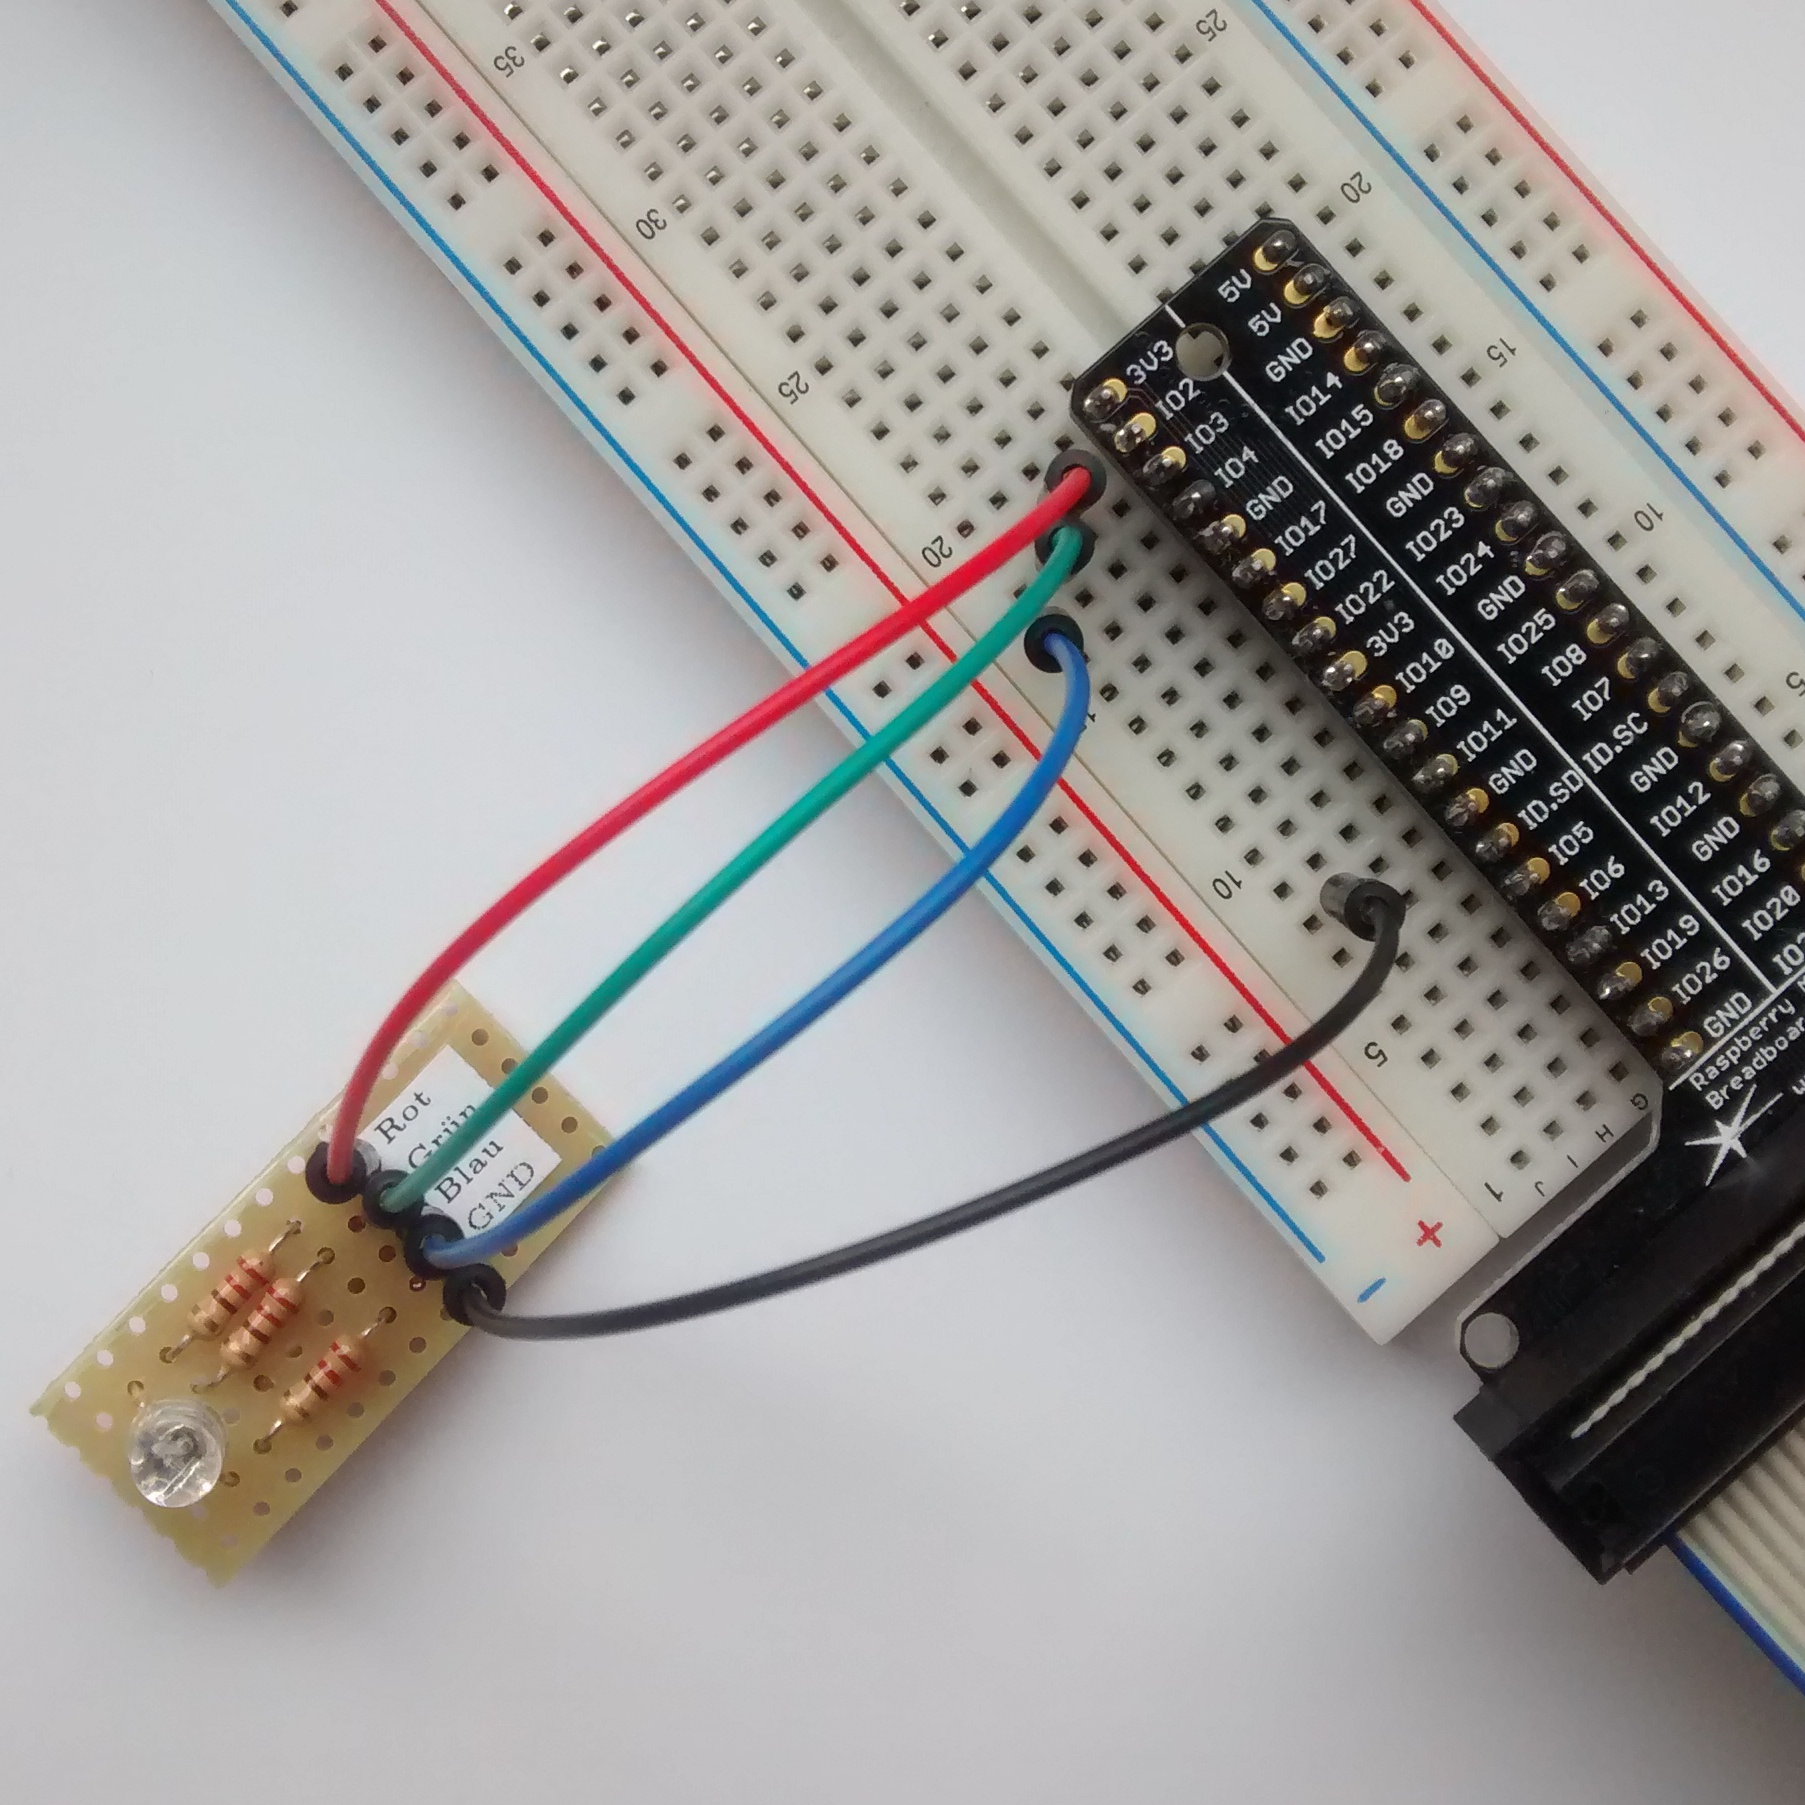
\includegraphics[width=0.49\textwidth]{img/anschluss_rgb_led}}
     \hfill
       \subfloat[Anschluss eines Helligkeitssensors (Anschluss an ">IO3"<, ">3V3"< und ">GND"<).]{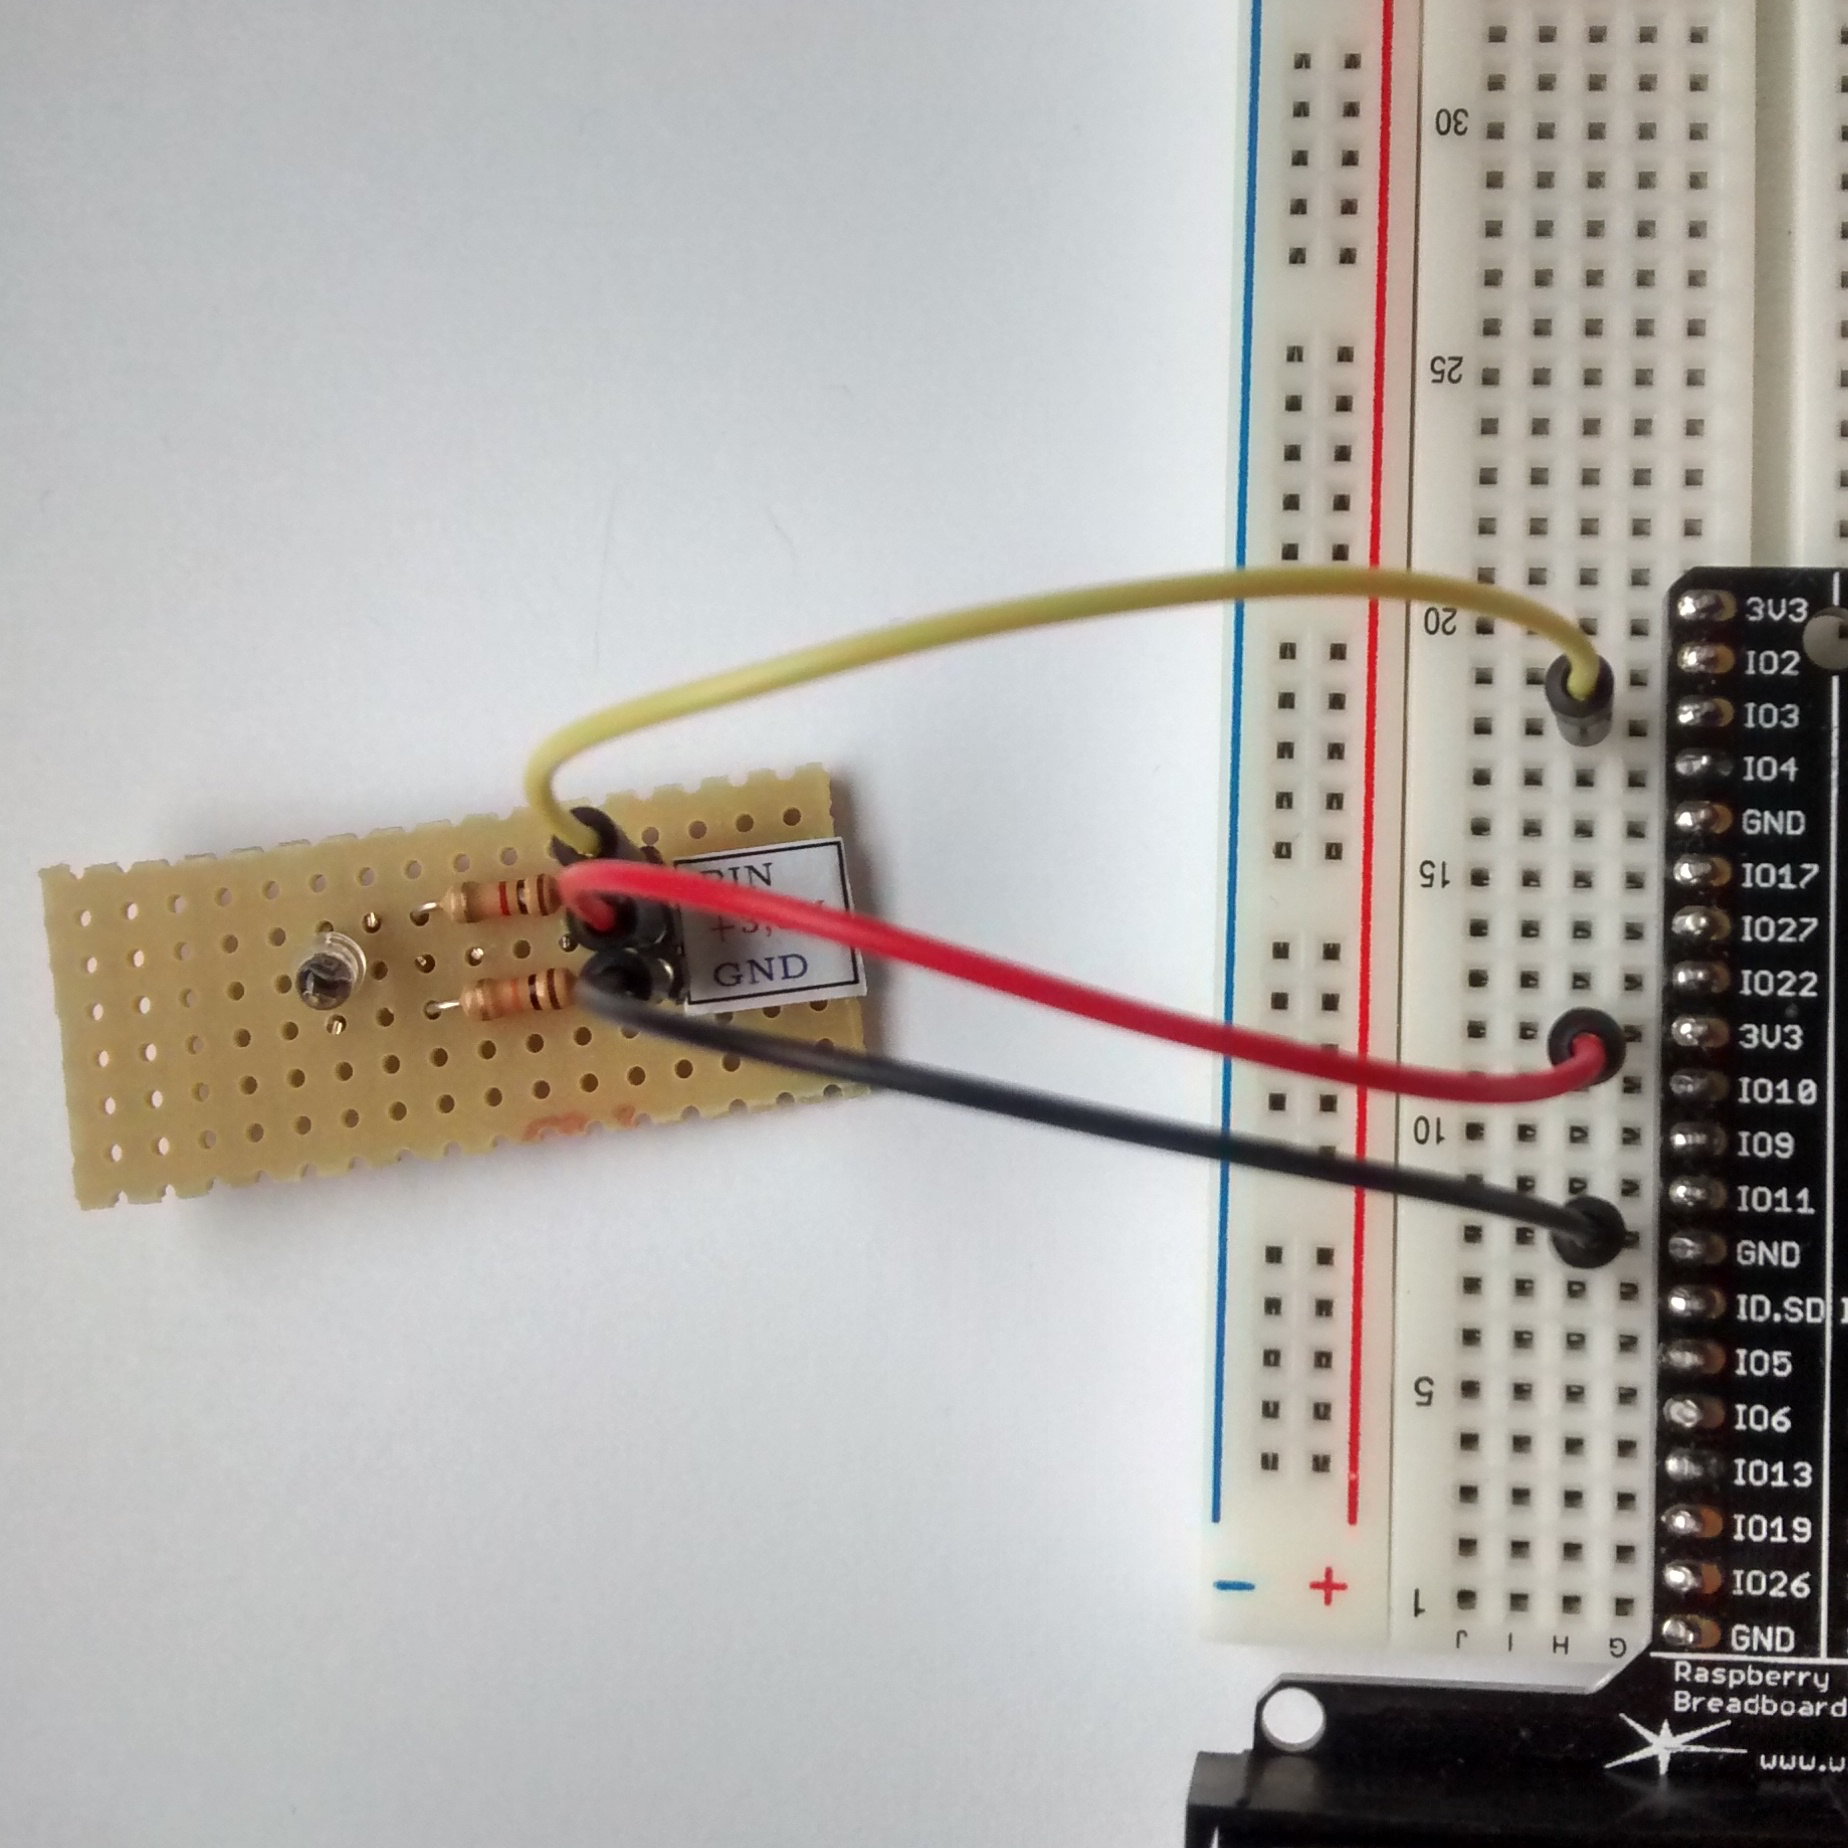
\includegraphics[width=0.49\textwidth]{img/anschluss_phototransistor}}
    \caption{Angeschlossene Objekte am Steckbrett.}
    \label{fig:objekte_steckbrett}
\end{figure*}

\subsection*{Abfolge zum Anschließen und Ansteuern eines Objektes}
\hinweis{Änderungen an der Hardware sollten nur dann erfolgen, wenn der Raspberry Pi ausgeschaltet ist.}

\begin{enumerate}

	\item Die Objekte mit Jumper-Kabeln mit dem GPIO des Raspberry Pi verbinden, die blaue Seite am Flachbandkabel muss dabei zum Displayanschluss zeigen. Anschließend die Objekte verkabeln.

	\item Am eingeschalteten Raspberry Pi die GroovyConsole starten: Dazu in einem geöffneten Terminalfenster folgendes eingeben:
		\begin{lstlisting}[gobble=6,language=Bash]
			cd rpCollection
			git pull
			./start.sh
		\end{lstlisting}

	Der erste Befehl wechselt in das passende Verzeichnis und der zweite aktualisiert die Daten, wenn eine Verbindung mit dem Internet besteht. Die Aktualisierung ist nur bei Bedarf notwendig.

	\item In der GroovyConsole können die Objekte direkt angesprochen werden. Im Quelltext \ref{listing:einfache_led} ist dazu ein Beispiel zum Schalten eines Scheinwerfers (einer LED) am Pin 11 angeben. 

		\begin{lstlisting}[caption={Steuerung eines Scheinwerfers.},label={listing:einfache_led}, gobble=6]
			gelbeLampe = new Scheinwerfer(11);
			gelbeLampe.anschalten();
			gelbeLampe.setzeStandort("Martins Buehne");
			sleep(400); //Warten von 400 Millisekunden = 0,4 Sekunden
			
			Helfer.herunterfahren(); //Pinne wieder frei geben (damit das Skript neu gestartet werden kann)
		\end{lstlisting}

	\item Die weiteren Methoden der Objekte stimmen mit denen aus dem Unterricht überein.

\end{enumerate}

\begin{aufgabe}
	Modelliere den Ablauf aus der Problembeschreibung aus der Sicht von Martin.
\end{aufgabe}



% Folgendes evtl. in eigene Datei auslagern:
%
%     Tabelle des GPIO-Controllers
%
%\newpage
%\begin{table}[htb]
%\centering
%\scalebox{1}{
%\begin{tabular}{>{\columncolor[gray]{1}}ll|>{\columncolor[gray]{0.9}}c >{\columncolor[gray]{0.9}}c|rr}
%\multicolumn{1}{l}{} & \multicolumn{1}{l}{\textbf{BCM}} & \multicolumn{1}{c}{}  & \multicolumn{1}{c}{}  & \multicolumn{1}{r}{\textbf{BCM}} & \multicolumn{1}{r}{}   
%\vspace{3mm}\\
%\arrayrulecolor[gray]{0}
%\hhline{>{\arrayrulecolor[gray]{1}}-->{\arrayrulecolor[gray]{0}}|--|>{\arrayrulecolor[gray]{1}}--|}
%\arrayrulecolor[gray]{0}
%& 3V3 & $\bullet$ & $\bullet$ & 5V &  \\
%& IO2 & $\bullet$ & $\bullet$ & 5V & \\
%& IO3 & $\bullet$ & $\bullet$ & GND & \\
%& IO4 & $\bullet$ & $\bullet$ & IO14 &  \\
%& GND & $\bullet$ & $\bullet$ & IO15 &  \\
%& IO17 & $\bullet$ & $\bullet$ & IO18 &  \\
%& IO27 & $\bullet$ & $\bullet$ & GND &  \\
%& IO22 & $\bullet$ & $\bullet$ & IO23 &  \\
%& 3V3 & $\bullet$ & $\bullet$ & IO24 &  \\
%& IO10 & $\bullet$ & $\bullet$ & GND &  \\
%& IO9 & $\bullet$ & $\bullet$ & IO25 &  \\
%& IO11 & $\bullet$ & $\bullet$ & IO8 &  \\
%& GND & $\bullet$ & $\bullet$ & IO7 &  \\
%& ID.SD & $\bullet$ & $\bullet$ & ID.SC &  \\
%& IO5 & $\bullet$ & $\bullet$ & GND &  \\
%& IO6 & $\bullet$ & $\bullet$ & IO12 &  \\
%& IO13 & $\bullet$ & $\bullet$ & GND &  \\
%& IO19 & $\bullet$ & $\bullet$ & IO16 &  \\
%& IO26 & $\bullet$ & $\bullet$ & IO20 & \\
%& GND & $\bullet$ & $\bullet$ & IO21 & \\
%\hhline{--|>{\arrayrulecolor[gray]{0.9}}-->{\arrayrulecolor{black}}|--|}
%\rowcolor[gray]{0.9}
%\multicolumn{1}{|c}{} & \multicolumn{1}{c}{}  & \multicolumn{1}{c}{} & \multicolumn{1}{c}{} & \multicolumn{1}{c}{} & \multicolumn{1}{c|}{} \\
%\hline
%\end{tabular}
%}
%\caption{Pin-Belegung auf dem GPIO (BCM-Layout).}
%\label{table:pinb_legung_bcm}
%\end{table}

\end{document}